% !TEX encoding = UTF-8 Unicode 

%MODIFICARE VERSIONI DEI FILE!
\level{1}{Resoconto delle varie attività di
verifica - Fase PD} 
Sono riportati in questa appendice tutti i risultati
ottenuti nei momenti di verifica, stabiliti nel \insdoc{Piano di Progetto
v6.00} secondo la strategia di misurazione per il perseguimento della qualità
individuata nel presente documento.

	\level{2}{Verifica dei prodotti}
		\level{3}{Documenti}
		In questa sezione vengono riportati gli esiti delle attività di verifica svolte sui documenti. Esse sono di due tipi:
		\begin{itemize}
			\item verifiche manuali;
			\item verifiche automatizzate.
		\end{itemize}
			\level{4}{Verifiche manuali}
			Le attività di verifica manuale della documentazione prodotta sono state svolte in base alla procedura riguardante la verifica dei documenti, descritta nel documento \insdoc{Norme di Progetto v6.00}.
			La verifica manuale, durante questa fase, ha permesso di individuare soprattutto:
			\begin{itemize}
			\item errori nell'utilizzo della lingua inglese;
			\item errori concettuali.
			\end{itemize}
			Si riporta di seguito la quantità degli errori rilevati e risolti, per ciascuna tipologia, durante l'intera fase.
			\begin{table}[H]
				\centering
					\begin{tabu}{| l | c |} \hline
						Errori di inglese & 28\\ \hline
						Errori concettuali & 5 \\ \hline
					\end{tabu}
					\caption{Errori trovati tramite verifica manuale dei documenti durante la Fase PD}
			\end{table}
			Si può notare che gli errori concettuali trovati sono un numero inferiore rispetto alla fase precedente, questo è dovuto sia alla minore quantità di modifiche apportate ai documenti durante la \insphase{Fase PD}, sia ad un miglioramento da parte dei membri del team nella stesura della documentazione, grazie all'esperienza acquisita durante tutto l'arco del progetto.
			Si noti invece come vi sia, ancora, una notevole quantità di errori nell'uso della lingua inglese dovuti alla stesura dei commenti del codice ed alla stesura del documento \insdoc{Manuale utente v3.00}.

			\level{4}{Verifiche automatizzate}
			Le attività di verifica automatizzate sono state effettuate secondo le procedure e attraverso gli strumenti descritti nel documento \insdoc{Norme di Progetto v6.00}. Esse hanno permesso di rilevare diversi errori, che sono stati poi corretti, riguardanti le seguenti tipologie:
			\begin{itemize}
				\item ortografia errata;
				\item norme tipografiche non rispettate.
			\end{itemize}
			Di seguito è presentato un riassunto della quantità di errori trovati (e successivamente risolti) utilizzando la verifica automatica.	
			\begin{table}[H]
				\centering
					\begin{tabu}{| l | c |}
						\hline
						Errori ortografici	& 82	\\ \hline
						Errori riguardanti norme tipografiche	& 5	\\ \hline
					\end{tabu}
				\caption{Errori trovati tramite verifica automatica dei documenti durante la Fase PD}
			\end{table}
			Da questi risultati si può notare il continuo miglioramento della documentazione prodotta, rispetto alle fasi precedenti. Si nota, anche, che non sono più stati rilevati errori nell'uso di \LaTeX{}.

		\level{3}{Codice}
		In questa sezione sono riportati i risultati delle metriche, calcolati nei momenti di verifica, per i tre prodotti: Norris, Chuck e applicazione Android.

			\level{4}{Numero di requisiti funzionali realizzati}
				\level{5}{Numero di requisiti funzionali obbligatori realizzati}
				Si riportano di seguito le percentuali di requisiti funzionali obbligatori realizzati dalle componenti di Norris.
				\begin{table}[H]
					\centering
						\begin{tabu}{| l | c | c |}
							\hline
							Componente	& Percentuale requisiti funzionali obbligatori soddisfatti	& Esito		\\ \hline \hline
							InternalAPIManager	& 100\% 	& Ottimale  \\ \hline
							ExternalAPIManager  & 	100\%	& Ottimale  \\ \hline
							DataModel  & 	100\%	& Ottimale  \\ \hline
						\end{tabu}
					\caption{Esiti del calcolo delle percentuali di requisiti funzionali obbligatori realizzati da Norris durante la Fase PD}
				\end{table}
				Come è possibile notare dalla tabella, la percentuale dei requisiti funzionali obbligatori soddisfatti da Norris ha raggiunto un esito complessivamente ottimale. 
				\\ \\
				Si riportano di seguito le percentuali di requisiti funzionali obbligatori realizzati dalle componenti di Chuck.
				\begin{table}[H]
					\centering
						\begin{tabu}{| l | c | c |}
							\hline
							Componente	& Numero requisiti funzionali obbligatori soddisfatti	& Esito		\\ \hline \hline
							Directive  &	100\% 	& Ottimale  \\ \hline
							ChartView  & 	100\%	& Ottimale  \\ \hline
							ViewModel  & 	100\%	& Ottimale  \\ \hline
							DataModel  & 	100\%	& Ottimale  \\ \hline
						\end{tabu}
					\caption{Esiti del calcolo delle percentuali di requisiti funzionali obbligatori realizzati da Chuck durante la Fase PD}
				\end{table}
				Come è possibile notare dalla tabella, la percentuale dei requisiti funzionali obbligatori soddisfatti da Chuck ha raggiunto un esito complessivamente ottimale.
				\\ \\
				Si riportano di seguito le percentuali di requisiti funzionali obbligatori realizzati dalle componenti dell'Applicazione.
				\begin{table}[H]
					\centering
						\begin{tabu}{| l | c | c |}
							\hline
							Componente	& Numero requisiti funzionali soddisfatti	& Esito		\\ \hline \hline
							Model				&   100\% 	& Ottimale \\ \hline
							Model:NorrisChart	&   100\% 	& Ottimale  \\ \hline
							Model:Service 		& 	100\%	& Ottimale   \\ \hline
							Presenter  			& 	100\%	& Ottimale  \\ \hline
							View  				& 	100\%	& Ottimale  \\ \hline
						\end{tabu}
					\caption{Esiti del calcolo delle percentuali di requisiti funzionali obbligatori realizzati dell'Applicazione durante la Fase PD}
				\end{table}
				Come è possibile notare dalla tabella la percentuale dei requisiti funzionali obbligatori soddisfatti dell'Applicazione ha raggiunto un esito ottimale.

				\level{5}{Numero di requisiti desiderabili funzionali realizzati}
				Si riportano di seguito le percentuali di requisiti desiderabili funzionali realizzati dalle componenti di Norris.
				\begin{table}[H]
					\centering
						\begin{tabu}{| l | c | c |}
							\hline
							Componente			& 	Percentuale requisiti desiderabili funzionali soddisfatti	& Esito		\\ \hline \hline
							InternalAPIManager	& 	100\% 	& Accettabile  \\ \hline
							ExternalAPIManager  & 	100\%	& Accettabile  \\ \hline
							DataModel  			& 	100\%	& Ottimale  \\ \hline
						\end{tabu}
					\caption{Esiti del calcolo delle percentuali di requisiti desiderabili funzionali realizzati da Norris durante la Fase PD}
				\end{table}
				Come è possibile notare dalla tabella la percentuale dei requisiti desiderabili funzionali soddisfatti da Norris ha raggiunto un esito ottimale. 
				\\ \\
				Si riportano di seguito le percentuali di requisiti desiderabili funzionali realizzati dalle componenti di Chuck.
				\begin{table}[H]
					\centering
						\begin{tabu}{| l | c | c |}
							\hline
							Componente	& Numero requisiti desiderabili funzionali soddisfatti	& Esito		\\ \hline \hline
							Directive	&	100\% 	& Accettabile  \\ \hline
							ChartView	& 	100\%	& Accettabile  \\ \hline
							ViewModel	& 	100\%	& Accettabile  \\ \hline
							DataModel	& 	100\%	& Ottimale  	\\ \hline
						\end{tabu}
					\caption{Esiti del calcolo delle percentuali di requisiti desiderabili funzionali realizzati da Chuck durante la Fase PD}
				\end{table}
				Come è possibile notare dalla tabella la percentuale dei requisiti desiderabili funzionali soddisfatti da Chuck ha raggiunto un esito, nel complesso, ottimale.

				\level{5}{Numero di requisiti opzionali funzionali realizzati}
				Si riportano di seguito le percentuali di requisiti opzionali funzionali realizzati dalle componenti di Norris.
				% \begin{table}[H]
				% 	\centering
				% 		\begin{tabu}{| l | c | c |}
				% 			\hline
				% 			Componente	& Percentuale requisiti opzionali funzionali soddisfatti	& Esito		\\ \hline \hline
				% 			DataModel  			& 	0\%	& 	Non accettabile  \\ \hline
				% 		\end{tabu}
				% 	\caption{Esiti del calcolo delle percentuali di requisiti opzionali funzionali realizzati da Norris durante la Fase PD}
				% \end{table}
				\\ \\ 

				Si riportano di seguito le percentuali di requisiti opzionali funzionali realizzati dalle componenti di Chuck.
				% \begin{table}[H]
				% 	\centering
				% 		\begin{tabu}{| l | c | c |}
				% 			\hline
				% 			Componente	& Numero requisiti opzionali funzionali soddisfatti	& Esito		\\ \hline \hline
				% 			ViewModel  	& 	0\%	& Non accettabile  \\ \hline
				% 			DataModel  	& 	0\%	& Non accettabile  \\ \hline
				% 		\end{tabu}
				% 	\caption{Esiti del calcolo delle percentuali di requisiti opzionali funzionali realizzati da Chuck durante la Fase PD}
				% \end{table}

			\level{4}{Percentuale di test di robustezza effettuati}
			Nella tabella seguente, vengono riportate le percentuali dei test effettuati sui tre prodotti: Norris, Chuck e applicazione Android.
%CALCOLARE
			\level{4}{Copertura del codice}
%CALCOLARE
			\level{4}{Complessità ciclomatica, numero di statement per metodo e livello di annidamento}
			Per ogni classe (in particolare ogni metodo di ciascuna classe) di Chuck e Norris, sono indicati, nella seguente tabella, i valori calcolati per le tre metriche: complessità ciclomatica (indicata con C.C.), numero di statement per metodo (indicato con N.S.) e livello di annidamento (indicato con L.A.).
				
				\begin{longtabu} spread 1cm [c]{|p{11cm}|p{1cm}|p{1cm}|p{1cm}|}
	\hline
					\rowfont{\bf \centering}
					Classe.metodo &
					C.C. &
					N.S.  &
					L.A. \\
					\hline
					\endhead
            
					\parbox[t]{4cm}{Chuck::Model::NorrisChart::BarChartInPlaceUpdater.update} &
                2 &
                18 &
                3\\\hline \parbox[t]{4cm}{Chuck::Model::NorrisChart::ChartImpl.createChart} &
                2 &
                5 &
                1\\\hline \parbox[t]{4cm}{Chuck::Model::NorrisChart::ChartImpl.getData} &
                1 &
                1 &
                0\\\hline \parbox[t]{4cm}{Chuck::Model::NorrisChart::ChartImpl.getId} &
                1 &
                1 &
                0\\\hline \parbox[t]{4cm}{Chuck::Model::NorrisChart::ChartImpl.getSettings} &
                1 &
                1 &
                0\\\hline \parbox[t]{4cm}{Chuck::Model::NorrisChart::ChartImpl.getType} &
                1 &
                1 &
                0\\\hline \parbox[t]{4cm}{Chuck::Model::NorrisChart::ChartImpl.setData} &
                1 &
                1 &
                0\\\hline \parbox[t]{4cm}{Chuck::Model::NorrisChart::ChartImpl.setSettings} &
                1 &
                4 &
                3\\\hline \parbox[t]{4cm}{Chuck::Model::NorrisChart::ChartImpl.update} &
                2 &
                7 &
                1\\\hline \parbox[t]{4cm}{Chuck::Model::NorrisChart::LineChartStreamUpdater.update} &
                4 &
                23 &
                6\\\hline \parbox[t]{4cm}{Chuck::Model::NorrisChart::LineChartInPlaceUpdater.update} &
                2 &
                18 &
                3\\\hline \parbox[t]{4cm}{Chuck::Model::NorrisChart::MapChartMovieUpdater.update} &
                1 &
                50 &
                6\\\hline \parbox[t]{4cm}{Chuck::Model::NorrisChart::MapChartInPlaceUpdater.update} &
                2 &
                19 &
                3\\\hline \parbox[t]{4cm}{Chuck::Model::NorrisChart::TableStreamUpdater.update} &
                6 &
                26 &
                5\\\hline \parbox[t]{4cm}{Chuck::Model::NorrisChart::TableInPlaceUpdater.update} &
                2 &
                19 &
                3\\\hline \parbox[t]{4cm}{Chuck::Model::Services::ChartRequester.bind} &
                1 &
                24 &
                1\\\hline \parbox[t]{4cm}{Chuck::ViewModel::BarChartViewModel.init} &
                1 &
                51 &
                2\\\hline \parbox[t]{4cm}{Chuck::ViewModel::BarChartViewModel.render} &
                1 &
                12 &
                2\\\hline \parbox[t]{4cm}{Chuck::ViewModel::LineChartViewModel.init} &
                1 &
                49 &
                2\\\hline \parbox[t]{4cm}{Chuck::ViewModel::LineChartViewModel.render} &
                1 &
                12 &
                1\\\hline \parbox[t]{4cm}{Chuck::ViewModel::MapChartViewModel.init} &
                1 &
                24 &
                1\\\hline \parbox[t]{4cm}{Chuck::ViewModel::MapChartViewModel.render} &
                1 &
                23 &
                2\\\hline \parbox[t]{4cm}{Chuck::ViewModel::TableViewModel.init} &
                1 &
                19 &
                1\\\hline \parbox[t]{4cm}{Chuck::ViewModel::TableViewModel.render} &
                1 &
                17 &
                2\\\hline \parbox[t]{4cm}{Norris::DataModel::NorrisChart::ChartImpl.getData} &
                1 &
                1 &
                0\\\hline \parbox[t]{4cm}{Norris::DataModel::NorrisChart::ChartImpl.getId} &
                1 &
                1 &
                0\\\hline \parbox[t]{4cm}{Norris::DataModel::NorrisChart::ChartImpl.getSettings} &
                1 &
                1 &
                0\\\hline \parbox[t]{4cm}{Norris::DataModel::NorrisChart::ChartImpl.getType} &
                1 &
                1 &
                0\\\hline \parbox[t]{4cm}{Norris::DataModel::NorrisChart::ChartImpl.setData} &
                1 &
                1 &
                0\\\hline \parbox[t]{4cm}{Norris::DataModel::NorrisChart::ChartImpl.setSettings} &
                2 &
                9 &
                4\\\hline \parbox[t]{4cm}{Norris::DataModel::NorrisChart::TableStreamUpdater.update} &
                6 &
                23 &
                6\\\hline \parbox[t]{4cm}{Norris::DataModel::NorrisChart::MapChartMovieUpdater.update} &
                5 &
                49 &
                5\\\hline \parbox[t]{4cm}{Norris::DataModel::NorrisChart::MapChartInPlaceUpdater.update} &
                3 &
                17 &
                3\\\hline \parbox[t]{4cm}{Norris::DataModel::NorrisChart::LineChartInStreamUpdater.update} &
                1 &
                1 &
                0\\\hline \parbox[t]{4cm}{Norris::DataModel::NorrisChart::LineChartInPlaceUpdater.update} &
                3 &
                16 &
                3\\\hline \parbox[t]{4cm}{Norris::DataModel::NorrisChart::ChartImpl.update} &
                2 &
                8 &
                1\\\hline \parbox[t]{4cm}{Norris::DataModel::NorrisChart::BarChartInPlaceUpdater.update} &
                1 &
                1 &
                0\\\hline \parbox[t]{4cm}{Norris::DataModel::NorrisChart::TableInPlaceUpdater.update} &
                3 &
                18 &
                3\\\hline \parbox[t]{4cm}{Norris::DataModel::NorrisImpl.createChart} &
                3 &
                8 &
                2\\\hline \parbox[t]{4cm}{Norris::DataModel::NorrisImpl.createPage} &
                2 &
                6 &
                1\\\hline \parbox[t]{4cm}{Norris::DataModel::NorrisImpl.getChart} &
                1 &
                1 &
                0\\\hline \parbox[t]{4cm}{Norris::DataModel::NorrisImpl.getCharts} &
                1 &
                1 &
                0\\\hline \parbox[t]{4cm}{Norris::DataModel::NorrisImpl.getPage} &
                1 &
                1 &
                0\\\hline \parbox[t]{4cm}{Norris::DataModel::NorrisImpl.getPages} &
                1 &
                1 &
                0\\\hline \parbox[t]{4cm}{Norris::DataModel::NorrisImpl.getSettings} &
                1 &
                1 &
                0\\\hline \parbox[t]{4cm}{Norris::DataModel::NorrisImpl.NorrisImpl} &
                2 &
                9 &
                1\\\hline \parbox[t]{4cm}{Norris::DataModel::NorrisImpl.setSettings} &
                1 &
                4 &
                3\\\hline \parbox[t]{4cm}{Norris::DataModel::NorrisPage::PageImpl.add} &
                4 &
                8 &
                2\\\hline \parbox[t]{4cm}{Norris::DataModel::NorrisPage::PageImpl.clearCharts} &
                1 &
                1 &
                0\\\hline \parbox[t]{4cm}{Norris::DataModel::NorrisPage::PageImpl.getCharts} &
                1 &
                1 &
                0\\\hline \parbox[t]{4cm}{Norris::DataModel::NorrisPage::PageImpl.getId} &
                1 &
                1 &
                0\\\hline \parbox[t]{4cm}{Norris::DataModel::NorrisPage::PageImpl.getSettings} &
                1 &
                1 &
                0\\\hline \parbox[t]{4cm}{Norris::DataModel::NorrisPage::PageImpl.setSettings} &
                1 &
                4 &
                3\\\hline \parbox[t]{4cm}{Norris::ExternalAPIManager::ChartRef.ChartRef} &
                2 &
                7 &
                1\\\hline \parbox[t]{4cm}{Norris::ExternalAPIManager::ChartRef.getData} &
                1 &
                1 &
                0\\\hline \parbox[t]{4cm}{Norris::ExternalAPIManager::ChartRef.getId} &
                1 &
                1 &
                0\\\hline \parbox[t]{4cm}{Norris::ExternalAPIManager::ChartRef.getSettings} &
                1 &
                1 &
                0\\\hline \parbox[t]{4cm}{Norris::ExternalAPIManager::ChartRef.getType} &
                1 &
                1 &
                0\\\hline \parbox[t]{4cm}{Norris::ExternalAPIManager::ExternalAPIConstructor.construct} &
                1 &
                3 &
                1\\\hline \parbox[t]{4cm}{Norris::ExternalAPIManager::ExternalAPIController.getChart} &
                1 &
                3 &
                0\\\hline \parbox[t]{4cm}{Norris::ExternalAPIManager::ExternalAPIController.getCharts} &
                1 &
                5 &
                1\\\hline \parbox[t]{4cm}{Norris::ExternalAPIManager::ExternalAPIConstructor.getInstance} &
                1 &
                1 &
                0\\\hline \parbox[t]{4cm}{Norris::ExternalAPIManager::ExternalAPIController.isLogged} &
                1 &
                3 &
                0\\\hline \parbox[t]{4cm}{Norris::ExternalAPIManager::ExternalAPIController.performKeepAlive} &
                1 &
                3 &
                0\\\hline \parbox[t]{4cm}{Norris::ExternalAPIManager::ExternalAPIController.performLogin} &
                1 &
                3 &
                0\\\hline \parbox[t]{4cm}{Norris::ExternalAPIManager::ExternalAPIController.performLogout} &
                1 &
                3 &
                0\\\hline \parbox[t]{4cm}{Norris::ExternalAPIManager::ExternalAPIConstructor.registerEndPoint} &
                1 &
                1 &
                0\\\hline \parbox[t]{4cm}{Norris::InternalAPIManager::ChartBridge.ChartBridge} &
                1 &
                2 &
                1\\\hline \parbox[t]{4cm}{Norris::InternalAPIManager::ChartBridge.getChartModel} &
                1 &
                1 &
                0\\\hline \parbox[t]{4cm}{Norris::InternalAPIManager::ChartBridge.getData} &
                1 &
                1 &
                0\\\hline \parbox[t]{4cm}{Norris::InternalAPIManager::ChartBridge.getId} &
                1 &
                1 &
                0\\\hline \parbox[t]{4cm}{Norris::InternalAPIManager::ChartBridge.getSettings} &
                1 &
                1 &
                0\\\hline \parbox[t]{4cm}{Norris::InternalAPIManager::ChartBridge.getType} &
                1 &
                1 &
                0\\\hline \parbox[t]{4cm}{Norris::InternalAPIManager::ChartBridge.setData} &
                1 &
                1 &
                0\\\hline \parbox[t]{4cm}{Norris::InternalAPIManager::ChartBridge.setSettings} &
                1 &
                1 &
                0\\\hline \parbox[t]{4cm}{Norris::InternalAPIManager::ChartBridge.update} &
                1 &
                1 &
                0\\\hline \parbox[t]{4cm}{Norris::InternalAPIManager::NorrisBridge.createChart} &
                1 &
                2 &
                0\\\hline \parbox[t]{4cm}{Norris::InternalAPIManager::NorrisBridge.createPage} &
                1 &
                2 &
                0\\\hline \parbox[t]{4cm}{Norris::InternalAPIManager::NorrisBridge.getChart} &
                1 &
                2 &
                0\\\hline \parbox[t]{4cm}{Norris::InternalAPIManager::NorrisBridge.getCharts} &
                1 &
                5 &
                0\\\hline \parbox[t]{4cm}{Norris::InternalAPIManager::NorrisBridge.getMiddleware} &
                1 &
                10 &
                1\\\hline \parbox[t]{4cm}{Norris::InternalAPIManager::NorrisBridge.getPage} &
                1 &
                2 &
                0\\\hline \parbox[t]{4cm}{Norris::InternalAPIManager::NorrisBridge.getPages} &
                1 &
                5 &
                0\\\hline \parbox[t]{4cm}{Norris::InternalAPIManager::NorrisBridge.getSettings} &
                1 &
                1 &
                0\\\hline \parbox[t]{4cm}{Norris::InternalAPIManager::NorrisBridge.setSettings} &
                1 &
                1 &
                0\\\hline \parbox[t]{4cm}{Norris::InternalAPIManager::PageBridge.add} &
                1 &
                3 &
                0\\\hline \parbox[t]{4cm}{Norris::InternalAPIManager::PageBridge.getCharts} &
                1 &
                5 &
                0\\\hline \parbox[t]{4cm}{Norris::InternalAPIManager::PageBridge.getId} &
                1 &
                1 &
                0\\\hline \parbox[t]{4cm}{Norris::InternalAPIManager::PageBridge.getSettings} &
                1 &
                1 &
                0\\\hline \parbox[t]{4cm}{Norris::InternalAPIManager::PageBridge.PageBridge} &
                1 &
                2 &
                1\\\hline \parbox[t]{4cm}{Norris::InternalAPIManager::PageBridge.setCharts} &
                1 &
                3 &
                0\\\hline \parbox[t]{4cm}{Norris::InternalAPIManager::PageBridge.setSettings} &
                1 &
                1 &
                0\\\hline                 \caption{Metodi e metriche Norris / Chuck}
				\end{longtabu}

			Per ogni classe (in particolare ogni metodo di ciascuna classe) diell'applicazione Android, sono indicati, nella seguente tabella, i valori calcolati per le tre metriche: complessità ciclomatica (indicata con C.C.), numero di statement per metodo (indicato con N.S.) e livello di annidamento (indicato con L.A.).
				
\begin{longtabu} spread 1cm [c]{|p{11cm}|p{1cm}|p{1cm}|p{1cm}|}
					\hline
					\rowfont{\bf \centering}
					Classe.metodo &
					C.C. &
					N.S.  &
					L.A. 
					\\
					\hline
					\endhead
            
					\parbox[t]{4cm}{Applicazione::Model::NorrisChart::ChartImpl.create} &
                1 &
                4 &
                1\\\hline \parbox[t]{4cm}{Applicazione::Model::NorrisChart::TableCell.getBackgroundColor} &
                1 &
                1 &
                0\\\hline \parbox[t]{4cm}{Applicazione::Model::NorrisChart::MapChartSettingsImpl.getCamera-\\ZoomHeight} &
                1 &
                4 &
                1\\\hline \parbox[t]{4cm}{Applicazione::Model::NorrisChart::ChartImpl.getData} &
                1 &
                1 &
                0\\\hline \parbox[t]{4cm}{Applicazione::Model::NorrisChart::LineChartDataImpl.getData} &
                1 &
                1 &
                0\\\hline \parbox[t]{4cm}{Applicazione::Model::NorrisChart::BarChartDataImpl.getData} &
                1 &
                1 &
                0\\\hline \parbox[t]{4cm}{Applicazione::Model::NorrisChart::TableDataImpl.getData} &
                1 &
                1 &
                0\\\hline \parbox[t]{4cm}{Applicazione::Model::NorrisChart::MapChartDataImpl.getData} &
                1 &
                1 &
                0\\\hline \parbox[t]{4cm}{Applicazione::Model::NorrisChart::TableRow.getData} &
                1 &
                1 &
                0\\\hline \parbox[t]{4cm}{Applicazione::Model::NorrisChart::MapSet.getData} &
                1 &
                1 &
                0\\\hline \parbox[t]{4cm}{Applicazione::Model::NorrisChart::TableCell.getData} &
                1 &
                1 &
                0\\\hline \parbox[t]{4cm}{Applicazione::Model::NorrisChart::TableStreamUpdate.getData} &
                1 &
                1 &
                0\\\hline \parbox[t]{4cm}{Applicazione::Model::NorrisChart::TableInPlaceUpdate.getData} &
                1 &
                1 &
                0\\\hline \parbox[t]{4cm}{Applicazione::Model::NorrisChart::MapChartInPlaceUpdate.getData} &
                1 &
                1 &
                0\\\hline \parbox[t]{4cm}{Applicazione::Model::NorrisChart::TableCellInPlaceUpdate.getData} &
                1 &
                1 &
                0\\\hline \parbox[t]{4cm}{Applicazione::Model::NorrisChart::MapChartElementInPlace-\\Update.getData} &
                1 &
                1 &
                0\\\hline \parbox[t]{4cm}{Applicazione::Model::NorrisChart::MapChartStreamUpdate.getData} &
                1 &
                1 &
                0\\\hline \parbox[t]{4cm}{Applicazione::Model::NorrisChart::MapChartDeleteUpdate.getData} &
                1 &
                1 &
                0\\\hline \parbox[t]{4cm}{Applicazione::Model::NorrisChart::LineChartStreamUpdate.getData} &
                1 &
                1 &
                0\\\hline \parbox[t]{4cm}{Applicazione::Model::NorrisChart::LineChartElementStream-\\Update.getData} &
                1 &
                1 &
                0\\\hline \parbox[t]{4cm}{Applicazione::Model::NorrisChart::BarChartInPlaceUpdate.getData} &
                1 &
                1 &
                0\\\hline \parbox[t]{4cm}{Applicazione::Model::NorrisChart::BarChartElementInPlace-\\Update.getData} &
                1 &
                1 &
                0\\\hline \parbox[t]{4cm}{Applicazione::Model::NorrisChart::LineChartInPlaceUpdate.getData} &
                1 &
                1 &
                0\\\hline \parbox[t]{4cm}{Applicazione::Model::NorrisChart::LineChartElementInPlace-\\Updater.getData} &
                1 &
                1 &
                0\\\hline \parbox[t]{4cm}{Applicazione::Model::NorrisChart::MapChartMovieUpdate.getDeleteData} &
                1 &
                1 &
                0\\\hline \parbox[t]{4cm}{Applicazione::Model::NorrisChart::TableCell.getFontColor} &
                1 &
                1 &
                0\\\hline \parbox[t]{4cm}{Applicazione::Model::NorrisChart::LineChartSettingsImpl.getGrid-\\Visibility} &
                1 &
                4 &
                1\\\hline \parbox[t]{4cm}{Applicazione::Model::NorrisChart::BarChartSettingsImpl.getGrid-\\Visibility} &
                1 &
                4 &
                1\\\hline \parbox[t]{4cm}{Applicazione::Model::NorrisChart::ChartImpl.getId} &
                1 &
                1 &
                0\\\hline \parbox[t]{4cm}{Applicazione::Model::NorrisChart::MapPoint.getId} &
                1 &
                1 &
                0\\\hline \parbox[t]{4cm}{Applicazione::Model::NorrisChart::MapChartElementInPlace-\\Update.getId} &
                1 &
                1 &
                0\\\hline \parbox[t]{4cm}{Applicazione::Model::NorrisChart::MapChartElementInPlace-\\Update.getIndex} &
                1 &
                1 &
                0\\\hline \parbox[t]{4cm}{Applicazione::Model::NorrisChart::MapChartElementInPlace-\\Update.getIndex} &
                1 &
                1 &
                0\\\hline \parbox[t]{4cm}{Applicazione::Model::NorrisChart::MapChartMovieUpdate.get-\\InPlaceData} &
                1 &
                1 &
                0\\\hline \parbox[t]{4cm}{Applicazione::Model::NorrisChart::TableDataImpl.getLabel} &
                1 &
                1 &
                0\\\hline \parbox[t]{4cm}{Applicazione::Model::NorrisChart::LineChartElement-\\StreamUpdate.getLabel} &
                1 &
                1 &
                0\\\hline \parbox[t]{4cm}{Applicazione::Model::NorrisChart::MapPoint.getLatitude} &
                1 &
                1 &
                0\\\hline \parbox[t]{4cm}{Applicazione::Model::NorrisChart::LineChartSettingsImpl.get-\\LegendPosition} &
                1 &
                1 &
                0\\\hline \parbox[t]{4cm}{Applicazione::Model::NorrisChart::BarChartSettingsImpl.get-\\LegendPosition} &
                1 &
                1 &
                0\\\hline \parbox[t]{4cm}{Applicazione::Model::NorrisChart::MapPoint.getLongitude} &
                1 &
                1 &
                0\\\hline \parbox[t]{4cm}{Applicazione::Model::NorrisChart::BarChartSettingsImpl.getOrientation} &
                1 &
                4 &
                1\\\hline \parbox[t]{4cm}{Applicazione::Model::NorrisChart::ChartImpl.getSettings} &
                1 &
                1 &
                0\\\hline \parbox[t]{4cm}{Applicazione::Model::NorrisChart::MapChartMovieUpdate.getStream-\\Data} &
                1 &
                1 &
                0\\\hline \parbox[t]{4cm}{Applicazione::Model::NorrisChart::ChartImpl.getType} &
                1 &
                1 &
                0\\\hline \parbox[t]{4cm}{Applicazione::Model::NorrisChart::TableCellInPlaceUpdate.getX} &
                1 &
                1 &
                0\\\hline \parbox[t]{4cm}{Applicazione::Model::NorrisChart::BarChartElementInPlace-\\Update.getX} &
                1 &
                1 &
                0\\\hline \parbox[t]{4cm}{Applicazione::Model::NorrisChart::LineChartElementInPlace-\\Updater.getX} &
                1 &
                1 &
                0\\\hline \parbox[t]{4cm}{Applicazione::Model::NorrisChart::LineChartSettingsImpl.getX-\\AxisName} &
                1 &
                4 &
                1\\\hline \parbox[t]{4cm}{Applicazione::Model::NorrisChart::BarChartSettingsImpl.getXAxisName} &
                1 &
                4 &
                1\\\hline \parbox[t]{4cm}{Applicazione::Model::NorrisChart::MapChartSettingsImpl.getXCamera-\\Coordinate} &
                1 &
                4 &
                1\\\hline \parbox[t]{4cm}{Applicazione::Model::NorrisChart::TableCellInPlaceUpdate.getY} &
                1 &
                1 &
                0\\\hline \parbox[t]{4cm}{Applicazione::Model::NorrisChart::BarChartElementInPlaceUpdate.getY} &
                1 &
                1 &
                0\\\hline \parbox[t]{4cm}{Applicazione::Model::NorrisChart::LineChartElementInPlace-\\Updater.getY} &
                1 &
                1 &
                0\\\hline \parbox[t]{4cm}{Applicazione::Model::NorrisChart::LineChartSettingsImpl.getYAxisName} &
                1 &
                4 &
                1\\\hline \parbox[t]{4cm}{Applicazione::Model::NorrisChart::BarChartSettingsImpl.getYAxisName} &
                1 &
                4 &
                1\\\hline \parbox[t]{4cm}{Applicazione::Model::NorrisChart::MapChartSettingsImpl.getYCamera-\\Coordinate} &
                1 &
                4 &
                1\\\hline \parbox[t]{4cm}{Applicazione::Model::NorrisChart::TableCell.setBackgroundColor} &
                1 &
                1 &
                0\\\hline \parbox[t]{4cm}{Applicazione::Model::NorrisChart::ChartImpl.setData} &
                1 &
                1 &
                0\\\hline \parbox[t]{4cm}{Applicazione::Model::NorrisChart::LineChartDataImpl.setData} &
                1 &
                1 &
                0\\\hline \parbox[t]{4cm}{Applicazione::Model::NorrisChart::BarChartDataImpl.setData} &
                1 &
                1 &
                0\\\hline \parbox[t]{4cm}{Applicazione::Model::NorrisChart::TableDataImpl.setData} &
                1 &
                1 &
                0\\\hline \parbox[t]{4cm}{Applicazione::Model::NorrisChart::MapChartDataImpl.setData} &
                1 &
                1 &
                0\\\hline \parbox[t]{4cm}{Applicazione::Model::NorrisChart::TableRow.setData} &
                1 &
                1 &
                0\\\hline \parbox[t]{4cm}{Applicazione::Model::NorrisChart::MapSet.setData} &
                1 &
                1 &
                0\\\hline \parbox[t]{4cm}{Applicazione::Model::NorrisChart::TableCell.setData} &
                1 &
                1 &
                0\\\hline \parbox[t]{4cm}{Applicazione::Model::NorrisChart::TableCell.setFontColor} &
                1 &
                1 &
                0\\\hline \parbox[t]{4cm}{Applicazione::Model::NorrisChart::MapPoint.setLatitude} &
                1 &
                1 &
                0\\\hline \parbox[t]{4cm}{Applicazione::Model::NorrisChart::MapPoint.setLongitude} &
                1 &
                1 &
                0\\\hline \parbox[t]{4cm}{Applicazione::Model::NorrisChart::ChartImpl.setSettings} &
                1 &
                4 &
                3\\\hline \parbox[t]{4cm}{Applicazione::Model::NorrisChart::TableInPlaceUpdater.update} &
                1 &
                4 &
                1\\\hline \parbox[t]{4cm}{Applicazione::Model::NorrisChart::BarChartInPlaceUpdater.update} &
                1 &
                1 &
                0\\\hline \parbox[t]{4cm}{Applicazione::Model::NorrisChart::ChartImpl.update} &
                1 &
                4 &
                1\\\hline \parbox[t]{4cm}{Applicazione::Model::NorrisChart::LineChartInPlaceUpdater.update} &
                1 &
                4 &
                1\\\hline \parbox[t]{4cm}{Applicazione::Model::NorrisChart::LineChartStreamUpdater.update} &
                2 &
                13 &
                2\\\hline \parbox[t]{4cm}{Applicazione::Model::NorrisChart::MapChartMovieUpdater.update} &
                1 &
                28 &
                4\\\hline \parbox[t]{4cm}{Applicazione::Model::NorrisChart::MapChartInPlaceUpdater.update} &
                1 &
                4 &
                1\\\hline \parbox[t]{4cm}{Applicazione::Model::NorrisChart::TableStreamUpdater.update} &
                1 &
                8 &
                2\\\hline \parbox[t]{4cm}{Applicazione::Model::NorrisSessionInfoImpl.getAddress} &
                1 &
                1 &
                0\\\hline \parbox[t]{4cm}{Applicazione::Model::NorrisSessionInfoImpl.getAuthCookie} &
                1 &
                1 &
                0\\\hline \parbox[t]{4cm}{Applicazione::Model::NorrisSessionInfoImpl.getInstance} &
                2 &
                3 &
                1\\\hline \parbox[t]{4cm}{Applicazione::Model::NorrisSessionInfoImpl.isLogged} &
                1 &
                1 &
                0\\\hline \parbox[t]{4cm}{Applicazione::Model::NorrisSessionInfoImpl.login} &
                1 &
                1 &
                0\\\hline \parbox[t]{4cm}{Applicazione::Model::NorrisSessionInfoImpl.logout} &
                1 &
                1 &
                0\\\hline \parbox[t]{4cm}{Applicazione::Model::NorrisSessionInfoImpl.setAddress} &
                1 &
                1 &
                0\\\hline \parbox[t]{4cm}{Applicazione::Model::Service::ChartReceiverImpl.getChart} &
                1 &
                14 &
                1\\\hline \parbox[t]{4cm}{Applicazione::Model::Service::ChartReceiverImpl.getInstance} &
                1 &
                3 &
                1\\\hline \parbox[t]{4cm}{Applicazione::Model::Service::ChartReceiverImpl.startUpdateEvent} &
                1 &
                4 &
                0\\\hline \parbox[t]{4cm}{Applicazione::Model::Service::ChartReceiverImpl.stopUpdateEvent} &
                1 &
                2 &
                0\\\hline \parbox[t]{4cm}{Applicazione::Presenter::BarChartPresenterImpl.applySettings} &
                1 &
                10 &
                0\\\hline \parbox[t]{4cm}{Applicazione::Presenter::BarChartPresenterImpl.update} &
                2 &
                21 &
                3\\\hline \parbox[t]{4cm}{Applicazione::Presenter::HttpRequesterWithCookie.getList} &
                1 &
                11 &
                1\\\hline \parbox[t]{4cm}{Applicazione::Presenter::HttpRequesterWithCookie.login} &
                1 &
                27 &
                1\\\hline \parbox[t]{4cm}{Applicazione::Presenter::HttpRequesterWithCookie.logout} &
                2 &
                7 &
                1\\\hline \parbox[t]{4cm}{Applicazione::Presenter::JSONParser.getInstance} &
                1 &
                3 &
                0\\\hline \parbox[t]{4cm}{Applicazione::Presenter::JSONParser.parseBarChart} &
                1 &
                25 &
                2\\\hline \parbox[t]{4cm}{Applicazione::Presenter::JSONParser.parseBarChartInPlaceUpdate} &
                1 &
                10 &
                1\\\hline \parbox[t]{4cm}{Applicazione::Presenter::JSONParser.parseBarChartSettings} &
                1 &
                1 &
                0\\\hline \parbox[t]{4cm}{Applicazione::Presenter::JSONParser.parseLineChart} &
                1 &
                25 &
                2\\\hline \parbox[t]{4cm}{Applicazione::Presenter::JSONParser.parseLineChartInPlaceUpdate} &
                1 &
                10 &
                1\\\hline \parbox[t]{4cm}{Applicazione::Presenter::JSONParser.parseLineChartSettings} &
                1 &
                1 &
                0\\\hline \parbox[t]{4cm}{Applicazione::Presenter::JSONParser.parseLineChartStreamUpdate} &
                1 &
                11 &
                2\\\hline \parbox[t]{4cm}{Applicazione::Presenter::JSONParser.parseMapChart} &
                1 &
                35 &
                2\\\hline \parbox[t]{4cm}{Applicazione::Presenter::JSONParser.parseMapChartDeleteUpdate} &
                1 &
                13 &
                2\\\hline \parbox[t]{4cm}{Applicazione::Presenter::JSONParser.parseMapChartInPlaceUpdate} &
                1 &
                24 &
                2\\\hline \parbox[t]{4cm}{Applicazione::Presenter::JSONParser.parseMapChartMovieUpdate} &
                1 &
                15 &
                1\\\hline \parbox[t]{4cm}{Applicazione::Presenter::JSONParser.parseMapChartSettings} &
                1 &
                1 &
                0\\\hline \parbox[t]{4cm}{Applicazione::Presenter::JSONParser.parseMapChartStreamUpdate} &
                1 &
                12 &
                2\\\hline \parbox[t]{4cm}{Applicazione::Presenter::JSONParser.parseTable} &
                1 &
                23 &
                3\\\hline \parbox[t]{4cm}{Applicazione::Presenter::JSONParser.parseTableInPlaceUpdate} &
                1 &
                19 &
                2\\\hline \parbox[t]{4cm}{Applicazione::Presenter::JSONParser.parseTableSettings} &
                1 &
                1 &
                0\\\hline \parbox[t]{4cm}{Applicazione::Presenter::JSONParser.parseTableStreamUpdate} &
                1 &
                19 &
                3\\\hline \parbox[t]{4cm}{Applicazione::Presenter::LineChartPresenterImpl.applySettings} &
                1 &
                9 &
                0\\\hline \parbox[t]{4cm}{Applicazione::Presenter::LineChartPresenterImpl.update} &
                4 &
                30 &
                3\\\hline \parbox[t]{4cm}{Applicazione::Presenter::ListPresenterImpl.onItemClicked} &
                1 &
                1 &
                0\\\hline \parbox[t]{4cm}{Applicazione::Presenter::ListPresenterImpl.onLogoutClick} &
                1 &
                2 &
                0\\\hline \parbox[t]{4cm}{Applicazione::Presenter::ListPresenterImpl.onResume} &
                1 &
                6 &
                0\\\hline \parbox[t]{4cm}{Applicazione::Presenter::LoginPresenterImpl.onLoginClick} &
                2 &
                7 &
                1\\\hline \parbox[t]{4cm}{Applicazione::Presenter::MapChartPresenterImpl.applySettings} &
                1 &
                4 &
                0\\\hline \parbox[t]{4cm}{Applicazione::Presenter::MapChartPresenterImpl.update} &
                4 &
                28 &
                3\\\hline \parbox[t]{4cm}{Applicazione::Presenter::PresenterImpl.create} &
                1 &
                3 &
                0\\\hline \parbox[t]{4cm}{Applicazione::Presenter::PresenterImpl.registerFactory} &
                1 &
                1 &
                0\\\hline \parbox[t]{4cm}{Applicazione::Presenter::TablePresenterImpl.applySettings} &
                1 &
                3 &
                0\\\hline \parbox[t]{4cm}{Applicazione::Presenter::TablePresenterImpl.update} &
                4 &
                28 &
                3\\\hline \parbox[t]{4cm}{Applicazione::View::BarChartActivity.onCreate} &
                1 &
                4 &
                0\\\hline \parbox[t]{4cm}{Applicazione::View::BarChartActivity.onPause} &
                1 &
                4 &
                0\\\hline \parbox[t]{4cm}{Applicazione::View::BarChartActivity.onResume} &
                1 &
                4 &
                0\\\hline \parbox[t]{4cm}{Applicazione::View::BarChartActivity.renderChart} &
                1 &
                11 &
                3\\\hline \parbox[t]{4cm}{Applicazione::View::BarChartActivity.setAxisName} &
                2 &
                6 &
                1\\\hline \parbox[t]{4cm}{Applicazione::View::BarChartActivity.setBarDataSetSpacing} &
                1 &
                3 &
                0\\\hline \parbox[t]{4cm}{Applicazione::View::BarChartActivity.setBarValueSpacing} &
                1 &
                4 &
                1\\\hline \parbox[t]{4cm}{Applicazione::View::BarChartActivity.setLegendPosition} &
                1 &
                13 &
                1\\\hline \parbox[t]{4cm}{Applicazione::View::BarChartActivity.setOrientation} &
                2 &
                12 &
                1\\\hline \parbox[t]{4cm}{Applicazione::View::BarChartActivity.showGrid} &
                1 &
                4 &
                0\\\hline \parbox[t]{4cm}{Applicazione::View::ChartActivity.getChartId} &
                1 &
                1 &
                0\\\hline \parbox[t]{4cm}{Applicazione::View::ChartActivity.getId} &
                1 &
                1 &
                0\\\hline \parbox[t]{4cm}{Applicazione::View::ChartActivity.renderChart} &
                0 &
                0 &
                0\\\hline \parbox[t]{4cm}{Applicazione::View::ChartActivity.setChartTitle} &
                1 &
                1 &
                0\\\hline \parbox[t]{4cm}{Applicazione::View::ChartActivity.setDescription} &
                1 &
                1 &
                0\\\hline \parbox[t]{4cm}{Applicazione::View::LineChartActivity.onCreate} &
                1 &
                4 &
                0\\\hline \parbox[t]{4cm}{Applicazione::View::LineChartActivity.onPause} &
                1 &
                4 &
                0\\\hline \parbox[t]{4cm}{Applicazione::View::LineChartActivity.onResume} &
                1 &
                4 &
                0\\\hline \parbox[t]{4cm}{Applicazione::View::LineChartActivity.renderChart} &
                1 &
                19 &
                0\\\hline \parbox[t]{4cm}{Applicazione::View::LineChartActivity.setAxisName} &
                1 &
                2 &
                0\\\hline \parbox[t]{4cm}{Applicazione::View::LineChartActivity.setCubicLines} &
                1 &
                4 &
                1\\\hline \parbox[t]{4cm}{Applicazione::View::LineChartActivity.setDotRadius} &
                1 &
                8 &
                2\\\hline \parbox[t]{4cm}{Applicazione::View::LineChartActivity.setDottedLines} &
                1 &
                7 &
                2\\\hline \parbox[t]{4cm}{Applicazione::View::LineChartActivity.setLegendPosition} &
                1 &
                13 &
                1\\\hline \parbox[t]{4cm}{Applicazione::View::LineChartActivity.setSeriesColor} &
                1 &
                1 &
                0\\\hline \parbox[t]{4cm}{Applicazione::View::LineChartActivity.showGrid} &
                1 &
                4 &
                0\\\hline \parbox[t]{4cm}{Applicazione::View::ListActivity.navigate} &
                1 &
                3 &
                0\\\hline \parbox[t]{4cm}{Applicazione::View::ListActivity.navigateToLoginView} &
                1 &
                3 &
                0\\\hline \parbox[t]{4cm}{Applicazione::View::ListActivity.onCreate} &
                1 &
                5 &
                0\\\hline \parbox[t]{4cm}{Applicazione::View::ListActivity.onItemClick} &
                1 &
                1 &
                0\\\hline \parbox[t]{4cm}{Applicazione::View::ListActivity.onLogoutClick} &
                1 &
                1 &
                0\\\hline \parbox[t]{4cm}{Applicazione::View::ListActivity.renderList} &
                1 &
                26 &
                2\\\hline \parbox[t]{4cm}{Applicazione::View::ListActivity.showChartDetailView} &
                1 &
                11 &
                1\\\hline \parbox[t]{4cm}{Applicazione::View::LoginActivity.onCreate} &
                1 &
                5 &
                0\\\hline \parbox[t]{4cm}{Applicazione::View::LoginActivity.onLoginClick} &
                1 &
                1 &
                0\\\hline \parbox[t]{4cm}{Applicazione::View::LoginActivity.showAuthenticationError} &
                1 &
                1 &
                0\\\hline \parbox[t]{4cm}{Applicazione::View::LoginActivity.showListView} &
                1 &
                2 &
                0\\\hline \parbox[t]{4cm}{Applicazione::View::LoginActivity.showProgress} &
                2 &
                4 &
                0\\\hline \parbox[t]{4cm}{Applicazione::View::MapChartActivity.onCreate} &
                1 &
                4 &
                0\\\hline \parbox[t]{4cm}{Applicazione::View::MapChartActivity.onPause} &
                1 &
                2 &
                0\\\hline \parbox[t]{4cm}{Applicazione::View::MapChartActivity.onResume} &
                1 &
                3 &
                0\\\hline \parbox[t]{4cm}{Applicazione::View::MapChartActivity.renderChart} &
                1 &
                18 &
                3\\\hline \parbox[t]{4cm}{Applicazione::View::MapChartActivity.setCameraCoordinate} &
                1 &
                1 &
                0\\\hline \parbox[t]{4cm}{Applicazione::View::MapChartActivity.setCameraZoom} &
                1 &
                1 &
                0\\\hline \parbox[t]{4cm}{Applicazione::View::MapChartActivity.setUpMapIfNeeded} &
                1 &
                4 &
                2\\\hline \parbox[t]{4cm}{Applicazione::View::TableActivity.onCreate} &
                1 &
                3 &
                0\\\hline \parbox[t]{4cm}{Applicazione::View::TableActivity.onPause} &
                1 &
                2 &
                0\\\hline \parbox[t]{4cm}{Applicazione::View::TableActivity.onResume} &
                1 &
                3 &
                0\\\hline \parbox[t]{4cm}{Applicazione::View::TableActivity.renderChart} &
                1 &
                24 &
                3\\\hline \parbox[t]{4cm}{Applicazione::View::TableActivity.showCellBorderLine} &
                2 &
                4 &
                1\\\hline                 \caption{Metodi e metriche applicazione}
				\end{longtabu}

			\level{4}{Numero di campi dati per classe}
%CALCOLARE
			\level{4}{Grado di accoppiamento dei componenti}
			Si riporta di seguito, per ogni componente, la percentuale del grado di accoppiamento afferente ed efferente.
%CALCOLARE appena progettazione completata, se no eliminare
			% \begin{table}[H]
			% 	\centering
			% 		\begin{tabu}{| l | c | c | c | c | c | c | }
			% 			\hline
			% 			Componente					& Afferente & Esiti Afferente & Efferente & Esiti Efferente 	\\ \hline \hline
			% 			Norris::InternalAPIManager	& 1 & Ottimale & 3 & Ottimale  \\ \hline
			% 			Norris::ExternalAPIManager  & 0 & Ottimale & 9 & Non Accettabile   \\ \hline
			% 			Norris::DataModel  			& 4 & Ottimale & 3 & Ottimale   \\ \hline
			% 			Chuck::Model 				& 2 & Ottimale & 4 & Ottimale   \\ \hline
			% 			Chuck::ViewModel 			& 8 & Non Accettabile & 6 & Accettabile   \\ \hline
			% 			Chuck::Directive 			& 0 & Ottimale & 12 & Non Accettabile   \\ \hline
			% 			Chuck::View 				& 4 & Ottimale & 4 & Ottimale   \\ \hline
			% 			App::Model 					& 3 & Ottimale & 2 & Ottimale   \\ \hline
			% 			App::Presenter 				& 3 & Ottimale & 6 & Accettabile   \\ \hline
			% 			App::View 					& 1 & Ottimale & 6 & Accettabile   \\ \hline
			% 		\end{tabu}
			% 	\caption{Esiti del calcolo del grado di accoppiamento per le componenti durante la Fase PD}
			% \end{table}
			% Come è possibile notare dalla tabella, abbiamo ottenuto buoni risultati sia per Norris sia per l'applicazione Android, mentre i valori del grado di accoppiamento afferente della componente ViewModel di Chuck sono risultati molto alti, in quanto rappresenta la componente principale di Chuck.
			 
	\level{2}{Verifica dei processi}
		\level{3}{Processo di documentazione}
			\level{4}{Livello CMM}
			In questa fase, il livello CMM del processo di documentazione si assesta al terzo gradino della scala CMM.

			\level{4}{Schedule Variance}
			La maggior parte delle attività pianificate nel \insdoc{Piano di Progetto v6.00}, relative alla documentazione, sono state svolte nei tempi previsti. \\
			Riportiamo di seguito i valori ottenuti calcolando la Schedule Variance sui tempi di stesura di ogni documento:
			\begin{table}[H]
					\centering
					\begin{tabu}{| l | c | c |}
							\hline
							Documenti 							& Schedule Variance	& Esito		\\ \hline \hline						
							Piano di progetto v6.00				& 4\% 		& Ottimale  \\ \hline
							Norme di Progetto v6.00 			& -1\%		& Ottimale  \\ \hline
							Piano di Qualifica v6.00 			& -1\%		& Accettabile  \\ \hline
							Manuale Utente v3.00 				& -2\%		& Ottimale  \\ \hline
							Definizione di Prodotto v3.00 		& -1\%		& Accettabile  \\ \hline
							Glossario v6.00					 	& 3\% 		& Ottimale  \\ \hline
							Totale processo di documentazione 	& 2\% 		& Accettabile \\ \hline
					\end{tabu}
				\caption{Esiti del calcolo della Schedule Variance durante la Fase PD}
			\end{table}
							
			\level{4}{Budget Variance}
%modificare, se pdp cambia, confrontare preventivo con consuntivo
			% Le risorse impiegate per la correzione degli errori e per l'avanzamento delle attività pianificate non hanno subito grosse modifiche rispetto a quanto pianificato. Questo deriva dal fatto che le modifiche apportate alla documentazione, in questa fase, sono state minime, mentre ci si è dedicati, in maggior misura, all'attività di codifica del codice sorgente e dei test e alla loro esecuzione.
			% Riportiamo di seguito i valori ottenuti calcolando la Budget Variance sulle risorse utilizzate per la stesura di ogni documento:
			% \begin{table}[H]
			% 		\centering
			% 		\begin{tabu}{| l | c | c |}
			% 				\hline
			% 				Documenti 							& Budget Variance	& Esito		\\ \hline \hline							
			% 				Piano di progetto v6.00				& 0\% 		& Ottimale  \\ \hline
			% 				Norme di Progetto v6.00 			& 0\%		& Accettabile  \\ \hline
			% 				Piano di Qualifica v6.00 			& 2\%		& Ottimale  \\ \hline
			% 				Specifica Tecnica v4.00 			& 0\%		& Ottimale  \\ \hline
			% 				Manuale Utente v3.00 				& -3\%		& Ottimale  \\ \hline
			% 				Definizione di Prodotto v3.00 		& -2\%		& Accettabile  \\ \hline
			% 				Glossario v6.00					 	& 3\% 		& Ottimale  \\ \hline
			% 				Totale processo di documentazione 	& 2\% 		& Ottimale \\ \hline
			% 		\end{tabu}
			% 	\caption{Esiti del calcolo della Budget Variance durante la Fase PD}
			% \end{table}
							
			\level{4}{Produttività}
			Utilizzando la formula descritta all'interno del presente documento (sezione \nameref{sec:metriche}) è stata calcolata la produttività del processo di documentazione. Questo indice è stato calcolato durante tutti i momenti di verifica previsti dal \insdoc{Piano di Progetto v6.00} per la \insphase{Fase PD}, per ogni documento redatto nel periodo antecedente la verifica. Il calcolo fatto di volta in volta sullo stesso documento tiene conto solo delle nuove sezioni introdotte in esso.\\
			Segue un riassunto di quanto è stato fatto.
			\begin{table}[H]
			      \centering
					\begin{tabu}{| l | c |}
					\hline
					Documento & Produttività	\\ \hline
					Norme di Progetto	& 20 \\ \hline
					Piano di Progetto	& 70 \\ \hline
					Piano di Qualifica	& 148 \\ \hline
					Definizione di Prodotto & 50 \\ \hline
					Manuale Utente & 150 \\ \hline
					Glossario & 80 \\ \hline
					\end{tabu}
					\caption{Produttività delle varie attività del processo di documentazione durante la fase PD}
			\end{table}
			Di seguito vengono riportati in un grafico i valori della produttività del processo di documentazione rilevati nei vari periodi della \insphase{Fase PD} nei quali è stato applicato il processo di verifica. Il grafico fa riferimento alla tabella precedente.\\

			\begin{figure}[H]
				\centering
					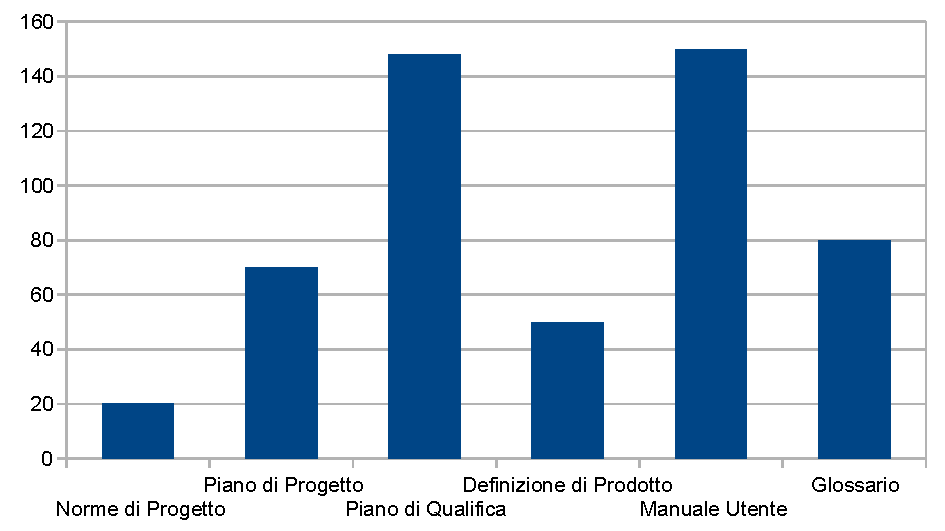
\includegraphics[width=12cm]{PianoDiQualifica/Pics/ProduttivitaDocumentazioneFasePD.pdf}
				\caption{Produttività del processo di documentazione durante la Fase PD}
			\end{figure}

			Si può notare come la produttività del processo di documentazione sia calato, rispetto alle fasi precedenti. Questo è dovuto al fatto che i docmenti hanno, ormai, raggiunto un buon livello di completezza dei contenuti. Sono, quindi, necessarie meno modifiche che abbassano il livello di produttività. \\
			Alcuni documenti presentano un indice di produttività più alto perchè hanno subito più modifiche ed incrementi.

		\level{3}{Processo di verifica}
			\level{4}{Livello CMM}
			In questa fase, il livello del processo di verifica si assesta al terzo gradino della scala CMM, già raggunto nella \insphase{Fase SD}.
			\level{4}{Schedule Variance}
			Il processo di verifica è stato sempre svolto rispettando le scadenze temporali previste nel \insdoc{Piano di Progetto v6.00}. I valori della Schedule Variance, calcolati per questo processo, risultano, quindi, ottimi.\\
			Riportiamo di seguito i valori ottenuti:
			\begin{table}[H]
				\centering
				\begin{tabu}{| l | c | c |}
					\hline
						Processi 			& Schedule Variance	& Esito		\\ \hline \hline
						Processo di verifica & 0\% & Ottimale \\ \hline
				\end{tabu}
				\caption{Esiti del calcolo della Schedule Variance durante la Fase PD}
			\end{table}	

			\level{4}{Budget Variance}
			Le risorse utilizzate nel processo di verifica sono di poco maggiori rispetto a qelle preventivate, a causa della necessità di correggere gli errori rilevati nella Revisione di Qualifica. Ciò ha causato un valore di poco inferiore alla soglia di accettabilità della Budget Variance.
			Riportiamo di seguito il valore ottenuto:
			\begin{table}[H]
				\centering
				\begin{tabu}{| l | c | c |}
				\hline
				Processi 			& Budget Variance	& Esito		\\ \hline \hline
				Processo di verifica & -2\% & Non Accettabile \\ \hline
				\end{tabu}
				\caption{Esiti del calcolo della Budget Variance durante la Fase PD}
			\end{table}	

			\level{4}{Produttività}
			Utilizzando la formula descritta all'interno del presente documento (sezione \nameref{sec:metriche}) è stata calcolata la produttività del processo di verifica. Tale indice è stato calcolato in seguito a tutti i momenti di verifica previsti dal \insdoc{Piano di Progetto v6.00} per la \insphase{Fase PD}. Di seguito vengono riportati i valori calcolati e una loro rappresentazione grafica.
			\begin{table}[H]
				\centering
				\begin{tabu}{| c | c |}
					\hline
					Data verifica & Produttività\\ \hline \hline
					01-02/06 & 3 \\ \hline
					03-05/06 & 10 \\ \hline
					06-11/06 & 16 \\ \hline		
					11-16/06 & 5 \\ \hline	
				\end{tabu}
				\caption{Produttività del processo di verifica durante la fase PD}
			\end{table}


			\begin{figure}[H]
				\centering
				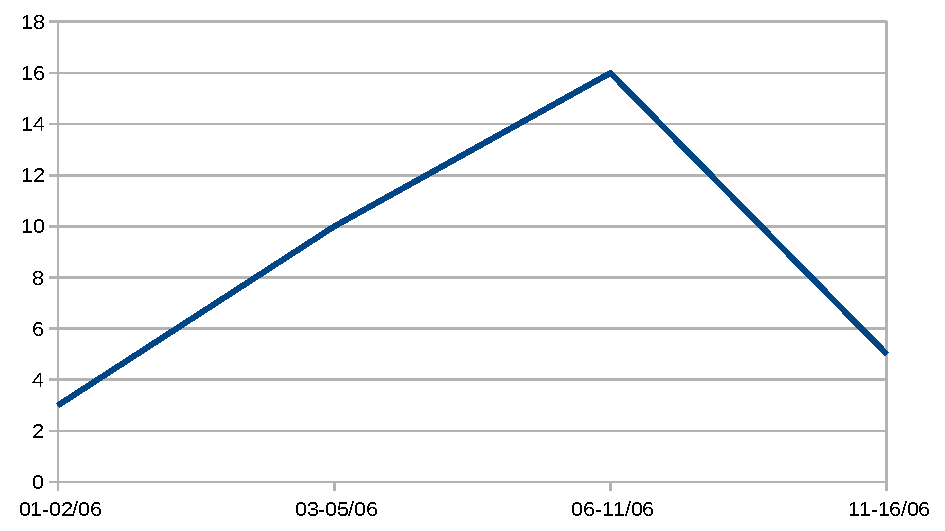
\includegraphics[width=12cm]{PianoDiQualifica/Pics/ProduttivitaVerificaFasePD.pdf}
				\caption{Produttività del processo di verifica durante la Fase PD}
			\end{figure}

			La produttività ha avuto un picco finale dovuto alla necessità di rivedere i documenti presentati alla Revisione di Qualifica, in seguito alle valutazioni ricevute, e alla necessità di verificare il codice prodotto. Si può notare che il livello di produttività è, in media, minore rispetto alle fasi precedenti, questo è dovuto, sempre, al fatto che sono state apportate meno modifiche ai documenti rispetto alle fasi precedenti.

			\level{4}{Efficacia di una revisione}
			Utilizzando la formula descritta all'interno del presente documento (sezione \nameref{sec:metriche}) è stata calcolata l'efficacia delle varie revisioni che sono state fatte durante la \insphase{Fase PD}. Di seguito vengono riportati i valori calcolati ed una loro rappresentazione grafica.
			\begin{table}[H]
				\centering
				\begin{tabu}{| c | c |}
					\hline
						Data verifica & Efficacia\\ \hline \hline
						01-02/06 & 6 \\ \hline
						03-05/06 & 10 \\ \hline
						06-11/06 & 18 \\ \hline		
						12-16/06 & 8 \\ \hline		
					\end{tabu}
				\caption{Efficacia delle revisioni durante la fase PD}
			\end{table}

			\begin{figure}[H]
				\centering
				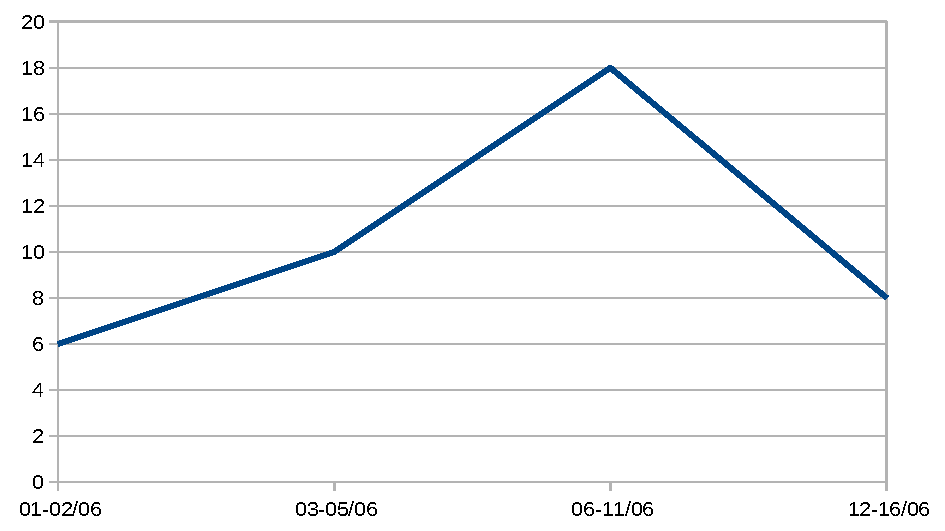
\includegraphics[width=12cm]{PianoDiQualifica/Pics/EfficaciaRevisioniFasePD.pdf}
				\caption{Efficacia delle revisioni durante la Fase PD}
			\end{figure}

			I livelli di efficacia di revisione, nel complesso, rispecchiano l'andamento della produttività. In generale, si ha una bassa efficacia, dovuta ad un basso numero di errori rilevati nei documenti ai quali sono state apportate modifiche. Vi è un picco nel momento in cui sono state apportate modifiche in seguito alle valutazioni ricevute dopo la Revisione di Qualifica.

		\level{3}{Processo di sviluppo}
		Si riportano, in questa sezione, gli esiti delle misurazioni effettuate rispetto all'attività di codifica.
			\level{4}{Livello CMM}
			Il gruppo \groupname{} conferma di aver raggiunto il terzo livello \insglo{CMM} anche per la parte del processo di sviluppo, relativa alla codifica. Il breve periodo, intercorso tra la fine della fase precedente e la fine della fase corrente, non ha permesso di ricercare i miglioramenti necessari a far aumentare la qualità del processo; il gruppo di lavoro si ritiene tuttavia soddisfatto del livello raggiunto nel processo.
				
			\level{4}{Schedule Variance}
			In questa fase la codifica è stata una delle attività principali a cui il gruppo si è dedicato. Nel complesso, il team, è riuscito a rispettare la pianificazione indicata nel \insdoc{Piano di Progetto v6.00}. Riportiamo di seguito i valori ottenuti calcolando la Schedule Variance sui tempi di stesura del codice sorgente.
			\begin{table}[H]
				\centering
				\begin{tabu}{| l | c | c |}
					\hline
						Processi 						& Schedule Variance	& Esito		\\ \hline \hline
						Processo di sviluppo (codifica) & -2\% & Accettabile \\ \hline
				\end{tabu}
				\caption{Esiti del calcolo della Schedule Variance durante la Fase PD}
			\end{table}	
						
			\level{4}{Budget Variance}
			Conseguentemente ai ritardi conseguiti nella fase precedente, le risorse impiegate sono state maggiori del previsto, al punto da richiedere la redistribuzione del monte ore totale fra i ruoli, come indicato nel \insdoc{Piano di Progetto v6.00}, e da sforare i range di accettazione della metrica.
%CALCOLARE, dopo pdp
			% \\
			% \begin{table}[H]
			% 	\centering
			% 	\begin{tabu}{| l | c | c |}
			% 		\hline
			% 			Processi 						& Budget Variance	& Esito		\\ \hline \hline
			% 			Processo di sviluppo (codifica) & -7\% & Non accettabile \\ \hline
			% 	\end{tabu}
			% 	\caption{Esiti del calcolo della Budget Variance dell'attività di codifica durante la Fase PD}
			% \end{table}	
							
			\level{4}{Produttività}
			Utilizzando la formula descritta all'interno del presente documento (sezione \nameref{sec:metriche}) è stata calcolata la produttività del processo di sviluppo, limitatamente all'attività di codifica. \\
			Seguono i risultati delle misurazioni.
			\\ 
			\begin{table}[H]
				\centering
				\begin{tabu}{| l | c | c |}
					\hline
						Processi 						& Produttività		\\ \hline \hline
						Processo di sviluppo (codifica) & 60   \\ \hline
				\end{tabu}
				\caption{Esiti del calcolo della produttività della codifica durante la Fase PD}
			\end{table}	
					
		\level{3}{PDCA}
		In questa sezione viene riportato il grafico PDCA della \insphase{Fase PD}. In ascissa è rappresentato il tempo, in ordinata le attività.

		% \begin{figure}[H]
		% 	\centering
		% 	\includegraphics[width=0.6\textwidth]{PianoDiQualifica/Pics/GraficoPDCAFasePD.png}
		% 	\caption{PDCA Fase PD}
		% \end{figure}

		Si può facilmente notare come la pianificazione non abbia subito grosse modifiche, rispetto a quanto preventivato. Vi è, quindi, un miglioramento, rispetto alla fase precedente, imputabile all'esperienza acquisita da parte del gruppo e ai pochi incrementi e cambiamenti da apportare ai vari documenti.